
%%%%%%%%%%%%%%%%%%%%%
\section{Force magnétique}
%%%%%%%%%%%%%%%%%%%%%
%

La force magnétique est la force qui s'exerce entre les \textbf{\textit {aimants}}.
Les aimants sont des matériaux possédant des propriétés magnétiques.
Certain métaux peuvent être aimantés par la proximité d'un aimant.

\subsection{Pôles magnétiques}

Un aimant est toujours {\it orienté}, il possède un pôle dit \textbf{\textit {nord}} et un pôle
dit \textbf{\textit {sud}}.


\subsection{Action magnétique}

La force magnétique entre deux aimants est attractive et répulsive, elle exerce un {\it couple} :
entre deux aimants, les pôles opposés s'attirent, les pôles identiques se repoussent. 

Ci-dessous, deux aimants sont schématisés, les pôles nord en rouge et les pôles sud en bleu. On ne représente que les forces que l'aimant 2 exerce sur l'aimant 1.

\begin{center}
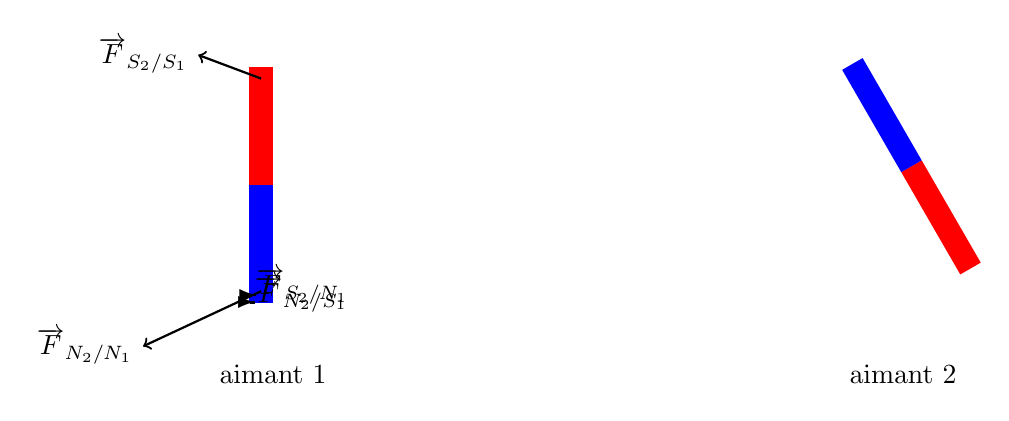
\begin{tikzpicture}[scale=1]
\fill [blue] (0,0) rectangle (0.3,1.5);
\fill [red] (0,1.5) rectangle (0.3,3);
\begin{scope}[rotate=30,yshift=-4.2cm]%
\fill [red] (8,0) rectangle (8.3,1.5);
\fill [blue] (8,1.5) rectangle (8.3,3);
\end{scope}
\thicklines
\put(0.15,0.15){\vector(1,0){1.76}}
\put(2,0.3){$\overrightarrow{F}_{N_2/S_1}$}

\put(0.15,2.85){\vector(1,0){2.26}}
\put(2.6,3){$\overrightarrow{F}_{S_2/N_1}$}

\draw [thick] [->] ((0.15,(0.15) --++(-1.5,-0.7) node [left] {$\overrightarrow{F}_{N_2/N_1}$};

\draw [thick] [->] ((0.15,(2.85) --++(-0.8,0.3) node [left] {$\overrightarrow{F}_{S_2/S_1}$};

\draw node at (0.3,-0.9) {aimant 1};
\draw node at (8.3,-0.9) {aimant 2};
\end{tikzpicture}
\end{center}
%%%%%%%%%%%%%%%%%%%%%%%%%%%%%%%%%%%%%%%%%%%%%%%%%%%%%%%%%%%%%%%%%%%%%%%%%%%%
